\documentclass[11pt,twoside,a4paper,openright]{report}
%%%%%%%%%%%%%%%%%%%%%%%%%%%%%%%%%%%%%%%%%%%%%%%%
% Language, Encoding and Fonts
% http://en.wikibooks.org/wiki/LaTeX/Internationalization
%%%%%%%%%%%%%%%%%%%%%%%%%%%%%%%%%%%%%%%%%%%%%%%%
% Select encoding of your inputs. Depends on
% your operating system and its default input
% encoding. Typically, you should use
%   Linux  : utf8 (most modern Linux distributions)
%            latin1 
%   Windows: ansinew
%            latin1 (works in most cases)
%   Mac    : applemac
% Notice that you can manually change the input
% encoding of your files by selecting "save as"
% an select the desired input encoding. 
\usepackage[utf8]{inputenc}
% Make latex understand and use the typographic
% rules of the language used in the document.
\usepackage[english]{babel}
% Use the palatino font
\usepackage[sc]{mathpazo}
\linespread{1.05}         % Palatino needs more leading (space between lines)
% Choose the font encoding
\usepackage[T1]{fontenc}

%%%%%%%%%%%%%%%%%%%%%%%%%%%%%%%%%%%%%%%%%%%%%%%%
% Graphics and Tables
% http://en.wikibooks.org/wiki/LaTeX/Importing_Graphics
% http://en.wikibooks.org/wiki/LaTeX/Tables
% http://en.wikibooks.org/wiki/LaTeX/Colors
%%%%%%%%%%%%%%%%%%%%%%%%%%%%%%%%%%%%%%%%%%%%%%%%
% load a colour package
\usepackage{xcolor}
\definecolor{aaublue}{RGB}{33,26,82}% dark blue
% The standard graphics inclusion package
\usepackage{graphicx}
% Set up how figure and table captions are displayed
\usepackage{caption}
\captionsetup{%
  font=footnotesize,% set font size to footnotesize
  labelfont=bf % bold label (e.g., Figure 3.2) font
}
% Make the standard latex tables look so much better
\usepackage{array,booktabs}
% Enable the use of frames around, e.g., theorems
% The framed package is used in the example environment
\usepackage{framed}

% Adds support for full page background picture
\usepackage[contents={},color=gray]{background}
%\usepackage[contents=draft,color=gray]{background}

%%%%%%%%%%%%%%%%%%%%%%%%%%%%%%%%%%%%%%%%%%%%%%%%
% Mathematics
% http://en.wikibooks.org/wiki/LaTeX/Mathematics
%%%%%%%%%%%%%%%%%%%%%%%%%%%%%%%%%%%%%%%%%%%%%%%%
% Defines new environments such as equation,
% align and split 
\usepackage{amsmath}
% Adds new math symbols
\usepackage{amssymb}
% Use theorems in your document
% The ntheorem package is also used for the example environment
% When using thmmarks, amsmath must be an option as well. Otherwise \eqref doesn't work anymore.
\usepackage[framed,amsmath,thmmarks]{ntheorem}

%%%%%%%%%%%%%%%%%%%%%%%%%%%%%%%%%%%%%%%%%%%%%%%%
% Page Layout
% http://en.wikibooks.org/wiki/LaTeX/Page_Layout
%%%%%%%%%%%%%%%%%%%%%%%%%%%%%%%%%%%%%%%%%%%%%%%%
% Change margins, papersize, etc of the document
\usepackage[
  inner=28mm,% left margin on an odd page
  outer=41mm,% right margin on an odd page
  ]{geometry}
% Modify how \chapter, \section, etc. look
% The titlesec package is very configureable
\usepackage{titlesec}
\titleformat{\chapter}[display]{\normalfont\huge\bfseries}{\chaptertitlename\ \thechapter}{20pt}{\Huge}
\titleformat*{\section}{\normalfont\Large\bfseries}
\titleformat*{\subsection}{\normalfont\large\bfseries}
\titleformat*{\subsubsection}{\normalfont\normalsize\bfseries}
%\titleformat*{\paragraph}{\normalfont\normalsize\bfseries}
%\titleformat*{\subparagraph}{\normalfont\normalsize\bfseries}

% Clear empty pages between chapters
\let\origdoublepage\cleardoublepage
\newcommand{\clearemptydoublepage}{%
  \clearpage
  {\pagestyle{empty}\origdoublepage}%
}
\let\cleardoublepage\clearemptydoublepage

% Change the headers and footers
\usepackage{fancyhdr}
\pagestyle{fancy}
\fancyhf{} %delete everything
\renewcommand{\headrulewidth}{0pt} %remove the horizontal line in the header
\fancyhead[RE]{\small\nouppercase\leftmark} %even page - chapter title
\fancyhead[LO]{\small\nouppercase\rightmark} %uneven page - section title
\fancyhead[LE,RO]{\thepage} %page number on all pages
% Do not stretch the content of a page. Instead,
% insert white space at the bottom of the page
\raggedbottom
% Enable arithmetics with length. Useful when
% typesetting the layout.
\usepackage{calc}

%%%%%%%%%%%%%%%%%%%%%%%%%%%%%%%%%%%%%%%%%%%%%%%%
% Bibliography
% http://en.wikibooks.org/wiki/LaTeX/Bibliography_Management
%%%%%%%%%%%%%%%%%%%%%%%%%%%%%%%%%%%%%%%%%%%%%%%%
\usepackage[backend=bibtex,
  bibencoding=utf8,
  style=numeric-comp
  ]{biblatex}
\addbibresource{bib/mybib}

%%%%%%%%%%%%%%%%%%%%%%%%%%%%%%%%%%%%%%%%%%%%%%%%
% Misc
%%%%%%%%%%%%%%%%%%%%%%%%%%%%%%%%%%%%%%%%%%%%%%%%
% Hide the ugly red borders around clickable hyperlinks/references
\usepackage[hidelinks]{hyperref}
% Add bibliography and index to the table of
% contents
\usepackage[nottoc]{tocbibind}
% Add the command \pageref{LastPage} which refers to the
% page number of the last page
\usepackage{lastpage}
% Add todo notes in the margin of the document
\usepackage[
%  disable, %turn off todonotes
  colorinlistoftodos, %enable a coloured square in the list of todos
  textwidth=\marginparwidth, %set the width of the todonotes
  textsize=scriptsize, %size of the text in the todonotes
  ]{todonotes}

%%%%%%%%%%%%%%%%%%%%%%%%%%%%%%%%%%%%%%%%%%%%%%%%
% Hyperlinks
% http://en.wikibooks.org/wiki/LaTeX/Hyperlinks
%%%%%%%%%%%%%%%%%%%%%%%%%%%%%%%%%%%%%%%%%%%%%%%%
% Enable hyperlinks and insert info into the pdf
% file. Hypperref should be loaded as one of the 
% last packages
\usepackage{hyperref}
\hypersetup{%
	pdfpagelabels=true,%
	plainpages=false,%
	pdfauthor={Author(s)},%
	pdftitle={Title},%
	pdfsubject={Subject},%
	bookmarksnumbered=true,%
	colorlinks=false,%
	citecolor=black,%
	filecolor=black,%
	linkcolor=black,% you should probably change this to black before printing
	urlcolor=black,%
	pdfstartview=FitH%
}

%%%%%%%%%%%%%%%%%%%%%%%%%%%%%%%%%%%%%%%%%%%%%%%%
% Listings (Code Snippets)
% https://en.wikibooks.org/wiki/LaTeX/Source_Code_Listings
%%%%%%%%%%%%%%%%%%%%%%%%%%%%%%%%%%%%%%%%%%%%%%%%
\usepackage{listings}
\usepackage{color}

\renewcommand{\lstlistingname}{Code Snippet} % Listing -> Code Snippet
\definecolor{lighter-gray}{RGB}{240,240,240}

\lstset{
  backgroundcolor=\color{lighter-gray},
  extendedchars=true,
  basicstyle=\footnotesize\ttfamily,
  showstringspaces=false,
  showspaces=false,
  numbers=left,
  tabsize=4,
  breaklines=true,
  showtabs=false,
  captionpos=b,
  numberstyle=\footnotesize,
  numbersep=5pt
}

% Define C# as a snippet language.
\usepackage{courier}

\definecolor{Green}{rgb}{0, 0.3, 0}
\definecolor{DarkCyan}{rgb}{0, 0.545, 0.545}
\definecolor{Navy}{rgb}{0, 0, 0.5}
\definecolor{Teal}{rgb}{0, 0.5, 0.5}
\definecolor{DarkGray}{gray}{0.66}
\definecolor{Olive}{rgb}{0.5, 0.5, 0}
\definecolor{Pink}{rgb}{1.0, 0.75, 0.8}
\definecolor{DeepPink}{rgb}{1, 0.08, 0.58}
\definecolor{Brown}{rgb}{0.65, 0.165, 0.165}
\definecolor{DarkViolet}{rgb}{0.58, 0, 0.83}
\definecolor{SaddleBrown}{rgb}{0.55, 0.27, 0.07}
\definecolor{Orange}{rgb}{0.9, 0.427, 0}
\lstdefinelanguage{CSharp}{
  morecomment = [l]{//}, 
  morecomment = [l]{///},
  morecomment = [s]{/*}{*/},
  morestring=[b]", 
  morestring=[b]',
  basicstyle=\footnotesize\ttfamily,
  commentstyle=\color{Green}\textit,
  stringstyle=\color{Orange},
  sensitive = true,
  morekeywords=[1]{this, base},
  keywordstyle=[1]\bfseries\color{Navy},
  morekeywords=[2]{as, is, new, sizeof, typeof, true, false, stackalloc},
  keywordstyle=[2]\color{Navy}\bfseries,
  morekeywords=[3]{else, if, switch, case, default,
  do, for, foreach, while, in},
  keywordstyle=[3]\bfseries\color{Navy} ,
  morekeywords=[4]{break, continue, goto, return,
  yield, partial, global, where},
  keywordstyle=[4]\bfseries\color{Navy},
  morekeywords=[5]{try, throw, catch, finally},
  keywordstyle=[5]\color{Navy}\bfseries,
  morekeywords=[6]{checked, unchecked},
  keywordstyle=[6]\color{Navy}\bfseries,
  morekeywords=[7]{fixed, unsafe},
  keywordstyle=[7]\bfseries\color{Navy},
  morekeywords=[8]{bool, byte, sbyte, char, short, ushort, int, uint, long, ulong, float,
  double, decimal, enum, struct},
  keywordstyle=[8]\bfseries\color{Navy},
  morekeywords=[9]{class, interface, delegate, object, string,
  void},
  keywordstyle=[9]\bfseries\color{Navy},
  morekeywords=[10]{explicit, implicit, operator},
  keywordstyle=[10]\bfseries\color{Navy},
  morekeywords=[11]{params, ref, out},
  keywordstyle=[11]\bfseries\color{Navy},
  morekeywords=[12]{private, protected, internal, public},
  keywordstyle=[12]\bfseries\color{Navy},
  morekeywords=[13]{abstract, const, event, var, override, virtual, volatile, extern, readonly, sealed, static},
  keywordstyle=[13]\bfseries\color{Navy},
  morekeywords=[14]{namespace, using},
  keywordstyle=[14]\bfseries\color{Navy},
  morekeywords=[15]{lock},
  keywordstyle=[15]\bfseries\color{Navy},
  morekeywords=[16]{get, set, add, remove},
  keywordstyle=[16]\bfseries\color{Navy},
  morekeywords=[17]{null, value},
  keywordstyle=[17]\bfseries\color{Navy},
}
\newcommand{\userStory}[3]{
  \begin{center}
    \begin{tabular}{|p{0.8\textwidth}|} 
     \hline
     \textbf{USER STORY}\\
     As \textit{#1}\\
     I want to be able to #2\\
     so I #3.\\ [0.5ex] 
     \hline
    \end{tabular}
    \end{center}  
    }
\usepackage{multirow}

\titleformat*{\subsubsection}{\large\bfseries}
\titleformat*{\subsection}{\Large\bfseries}
\titleformat*{\section}{\LARGE\bfseries}% package inclusion and set up of the document
% see, e.g., http://en.wikibooks.org/wiki/LaTeX/Formatting#Hyphenation
% for more information on word hyphenation
\hyphenation{ex-am-ple hy-phen-a-tion short}
\hyphenation{long la-tex}
% 
% see, e.g., http://en.wikibooks.org/wiki/LaTeX/Customizing_LaTeX#New_commands
% for more information on how to create macros

%%%%%%%%%%%%%%%%%%%%%%%%%%%%%%%%%%%%%%%%%%%%%%%%
% Macros for the titlepage
%%%%%%%%%%%%%%%%%%%%%%%%%%%%%%%%%%%%%%%%%%%%%%%%
%Creates the aau titlepage
\newcommand{\aautitlepage}[3]{%
  {
    %set up various length
    \ifx\titlepageleftcolumnwidth\undefined
      \newlength{\titlepageleftcolumnwidth}
      \newlength{\titlepagerightcolumnwidth}
    \fi
    \setlength{\titlepageleftcolumnwidth}{0.5\textwidth-\tabcolsep}
    \setlength{\titlepagerightcolumnwidth}{\textwidth-2\tabcolsep-\titlepageleftcolumnwidth}
    %create title page
    \thispagestyle{empty}
    \noindent%
    \begin{tabular}{@{}ll@{}}
      \parbox{\titlepageleftcolumnwidth}{
        \iflanguage{danish}{%
          
\includegraphics[width=\titlepageleftcolumnwidth]{AAUgraphics/aau_logo_da}
        }{%
          
\includegraphics[width=\titlepageleftcolumnwidth]{AAUgraphics/aau_logo_en}
        }
      } &
      \parbox{\titlepagerightcolumnwidth}{\raggedleft\sf\small
        #2
      }\bigskip\\
       #1 &
      \parbox[t]{\titlepagerightcolumnwidth}{%
      \textbf{Abstract:}\bigskip\par
        \fbox{\parbox{\titlepagerightcolumnwidth-2\fboxsep-2\fboxrule}{%
          #3
        }}
      }\\
    \end{tabular}
    \vfill
    \iflanguage{danish}{%
      \noindent{\footnotesize\emph{Rapportens indhold er frit tilgængeligt, men offentliggørelse (med kildeangivelse) må kun ske efter aftale med forfatterne.}}
    }{%
      \noindent{\footnotesize\emph{The content of this report is freely available, but publication (with reference) may only be pursued due to agreement with the author.}}
    }
    \clearpage
  }
}

%Create english project info
\newcommand{\englishprojectinfo}[8]{%
  \parbox[t]{\titlepageleftcolumnwidth}{
    \textbf{Title:}\\ #1\bigskip\par
    \textbf{Theme:}\\ #2\bigskip\par
    \textbf{Project Period:}\\ #3\bigskip\par
    \textbf{Project Group:}\\ #4\bigskip\par
    \textbf{Participant(s):}\\ #5\bigskip\par
    \textbf{Supervisor(s):}\\ #6\bigskip\par
    \textbf{Copies:} #7\bigskip\par
    \textbf{Page Numbers:} \pageref{LastPage}\bigskip\par
    \textbf{Date of Completion:}\\ #8
  }
}

%Create danish project info
\newcommand{\danishprojectinfo}[8]{%
  \parbox[t]{\titlepageleftcolumnwidth}{
    \textbf{Titel:}\\ #1\bigskip\par
    \textbf{Tema:}\\ #2\bigskip\par
    \textbf{Projektperiode:}\\ #3\bigskip\par
    \textbf{Projektgruppe:}\\ #4\bigskip\par
    \textbf{Deltager(e):}\\ #5\bigskip\par
    \textbf{Vejleder(e):}\\ #6\bigskip\par
    \textbf{Oplagstal:} #7\bigskip\par
    \textbf{Sidetal:} \pageref{LastPage}\bigskip\par
    \textbf{Afleveringsdato:}\\ #8
  }
}

%%%%%%%%%%%%%%%%%%%%%%%%%%%%%%%%%%%%%%%%%%%%%%%%
% An example environment
%%%%%%%%%%%%%%%%%%%%%%%%%%%%%%%%%%%%%%%%%%%%%%%%
\theoremheaderfont{\normalfont\bfseries}
\theorembodyfont{\normalfont}
\theoremstyle{break}
\def\theoremframecommand{{\color{gray!50}\vrule width 5pt \hspace{5pt}}}
\newshadedtheorem{exa}{Example}[chapter]
\newenvironment{example}[1]{%
		\begin{exa}[#1]
}{%
		\end{exa}
}

\newcommand{\knox}{Knox}
\newcommand{\postgres}{PostgreSQL}% my new macros

\begin{document}
%frontmatter
\pagestyle{empty} %disable headers and footers
\pagenumbering{roman} %use roman page numbering in the frontmatter
%\pdfbookmark[0]{Front page}{label:frontpage}%

\begin{titlepage}
\newgeometry{top=0cm,bottom=1.2cm,right=0cm,left=0cm}

  \backgroundsetup{
   scale=1.1,
   angle=0,
   opacity=1.0,  %% adjust
   contents={\includegraphics[width=\paperwidth,height=\paperheight]{AAUgraphics/aau_waves}}
    }
		
  \begin{center} %%please do not change the height or width of the frontpage image
    \centerline{
\includegraphics[totalheight=0.5\paperwidth,width=1\paperwidth]{AAUgraphics/frontpageImage}}% 
  \end{center}
	
	\vspace*{-0.96cm}
  {\noindent\color{aaublue}\fboxsep0pt\colorbox{white}{\begin{tabular}{@{}p{\paperwidth}@{}}
    \centerline{
    \begin{minipage}{0.85\textwidth}
        \bigskip
				\bigskip
        \centering
        \Huge{\textbf{
A simple explanation of how our Universe was formed% insert your title here
        }}
    \end{minipage}
    }
		
	\centerline{
	\begin{minipage}{0.9\textwidth}
        \bigskip
        \centering
        \Large{
Development of a predictive model% insert your subtitle here
        }
    \end{minipage}
    }
			
	\centerline{
	\begin{minipage}{0.9\textwidth}
        \bigskip
        \centering
        {\Large
Anders Andersen, Alfred Alfredsen, Anne Annesen% insert names separated by comma
        }
    \end{minipage}
    }
			
    \centerline{
    \begin{minipage}{0.9\textwidth}
        \bigskip
        \centering
        {\large
Energy Technology, TEPE4-1005, \the\year-06% insert name of study, group number, year-month
        } 
    \end{minipage}
    }
			
    \centerline{
    \begin{minipage}{0.9\textwidth}
        \bigskip
        \centering
%% Comment this section if you are not doing Bachelor or Master Project   
        {\Large
Master's Project
      %Bachelor Project
        }
        \smallskip
    \end{minipage}
    }
			
  \end{tabular}}}

  \vfill
  \begin{figure}[!b]
	\centering
    
\includegraphics[width=0.2\paperwidth]{AAUgraphics/aau_logo_circle_en}% comment this line in for English version
    %
\includegraphics[width=0.2\paperwidth]{AAUgraphics/aau_logo_circle_da} %comment this line in for Danish version
  \end{figure}
\end{titlepage}
\restoregeometry
\pdfbookmark[0]{Front page}{label:frontpage}%
\begin{titlepage}
\vspace*{\fill}
    \backgroundsetup{
    scale=1.1,
    angle=0,
    opacity=1.0,  %% adjust
    contents={\includegraphics[width=\paperwidth,height=\paperheight]{AAUgraphics/aau_waves}}
    }
  \addtolength{\hoffset}{0.5\evensidemargin-0.5\oddsidemargin} %set equal margins on the frontpage - remove this line if you want default margins
  \noindent%
  {\color{white}\fboxsep0pt\colorbox{aaublue}{\begin{tabular}{@{}p{\textwidth}@{}}
    \begin{center}
    \Huge{\textbf{
      A study on the Universe% insert your title here
    }}
    \end{center}
    \begin{center}
      \Large{
        Development of a predictive model% insert your subtitle here
      }
    \end{center}
    \vspace{0.2cm}
   \begin{center}
    {\Large
      Anders Andersen, Alfred Alfredsen, Anne Annesen% insert names separated by comma
    }\\
    \vspace{0.2cm}
    {\large
      Energy Technology, TEPE4-1005, 2018-06% insert name of study, group number, year-month
    }
   \end{center}
   \vspace{0.2cm}
%% Comment this section in if you are doing Bachelor or Master Project   
   \begin{center}
    {\Large
      Master's Project
      %Bachelor Project
    }
   \end{center}
  \end{tabular}}}
  \vfill
  \begin{center}
    
\includegraphics[width=0.2\paperwidth]{AAUgraphics/aau_logo_circle_en}% comment this line in for English version
    %
\includegraphics[width=0.2\paperwidth]{AAUgraphics/aau_logo_circle_da} %comment this line in for Danish version
  \end{center}
\end{titlepage}
\clearpage

\thispagestyle{empty}
{\small
\strut\vfill % push the content to the bottom of the page
\noindent Copyright \copyright{} Aalborg University 2015\par
\vspace{0.2cm}
\noindent Here you can write something about which tools and software you have used for typesetting the document, running simulations and creating figures. If you do not know what to write, either leave this page blank or have a look at the colophon in some of your books.\todo{Add a colophon}
}
\clearpage


\pdfbookmark[0]{English title page}{label:titlepage_en}
\aautitlepage{%
  \englishprojectinfo{
    Placeholder Title %title
  }{%
    Scientific Theme %theme
  }{%
    Fall Semester 2021 %project period
  }{%
    cs-21-sw-5-19 % project group
  }{%
    %list of group members
    Christian Bager Bach Houmann\\
    Daniel Overvad Nykjær\\
    Ivik Lau Dalgas Hostrup\\
    Marco Klaustrup Justesen\\
    Patrick Frostholm Østergaard\\
    Rasmus Høyer Hansen
  }{%
    %list of supervisors
    Christian Aebeloe
  }{%
    1 % number of printed copies
  }{%
    \today % date of completion
  }%
}{%department and address
  \textbf{Computer Science}\\
  Aalborg University\\
  \href{http://www.aau.dk}{http://www.aau.dk}
}{% the abstract
Knox (Knowledge Engineering Toolbox) is a continuous pipeline project involving several project groups working in scrum-inspired environment.
This report documents the work of the third layer of the pipeline, responsible for database and server management.
For the first half of the project, the groups collaborated on developing a search engine.
Here we designed and implemented database structures in the relational database management system PostgreSQL.
This report then documents this design and the implementation of the required API endpoints to access it using HTTP.
For the second half of the project, the groups began development of features based on knowledge graphs.
 Here we supported the other groups by implementing a data storage for the used RDF data. 
}

% \cleardoublepage
% {\selectlanguage{danish}
% \pdfbookmark[0]{Danish title page}{label:titlepage_da}
% \aautitlepage{%
%   \danishprojectinfo{
%     Rapportens titel %title
%   }{%
%     Semestertema %theme
%   }{%
%     Efterårssemestret 2010 %project period
%   }{%
%     XXX % project group
%   }{%
%     %list of group members
%     Forfatter 1\\ 
%     Forfatter 2\\
%     Forfatter 3
%   }{%
%     %list of supervisors
%     Vejleder 1\\
%     Vejleder 2
%   }{%
%     1 % number of printed copies
%   }{%
%     \today % date of completion
%   }%
% }{%department and address
%   \textbf{Elektronik og IT}\\
%   Aalborg Universitet\\
%   \href{http://www.aau.dk}{http://www.aau.dk}
% }{% the abstract
%   Her er resuméet
% }}
% 
\cleardoublepage
\pdfbookmark[0]{Contents}{label:contents}
\pagestyle{fancy} %enable headers and footers again
\tableofcontents
\listoftodos
\chapter*{Preface\markboth{Preface}{Preface}}\label{ch:preface}
\addcontentsline{toc}{chapter}{Preface}
Group cs-21-sw-5-19 will hereby referred to as \textit{our group}, \textit{our}, or \textit{we} for the purpose of this document.
This report is a documentation of the work done by our group in the course of the semester.

We would like to extend our thanks to our supervisor \textit{Christian} for the support and guidance that we received throughout the semester.

\vspace{\baselineskip}\hfill Aalborg University, \today
\vfill\noindent


\begin{minipage}[b]{0.45\textwidth}
 \centering
 \rule{\textwidth}{0.5pt}\\
 Christian Bager Bach Houmann\\
 {\footnotesize <chouma19@student.aau.dk>}
\end{minipage}

\hfill
\begin{minipage}[b]{0.45\textwidth}
 \centering
 \rule{\textwidth}{0.5pt}\\
  Daniel Overvad Nykjær\\
 {\footnotesize <dnykja18@student.aau.dk>}
\end{minipage}

\begin{minipage}[b]{0.45\textwidth}
 \centering
 \rule{\textwidth}{0.5pt}
  Ivik Lau Dalgas Hostrup\\
 {\footnotesize <ihostr16@student.aau.dk>}
\end{minipage}

\hfill
\begin{minipage}[b]{0.45\textwidth}
 \centering
 \rule{\textwidth}{0.5pt}
  Marco Klaustrup Justesen\\
 {\footnotesize <mkju19@student.aau.dk>}
\end{minipage}

\begin{minipage}[b]{0.45\textwidth}
 \centering
 \rule{\textwidth}{0.5pt}
  Patrick Frostholm Østergaard\\
 {\footnotesize <pfas19@student.aau.dk>}
\end{minipage}

\hfill
\begin{minipage}[b]{0.45\textwidth}
 \centering
 \rule{\textwidth}{0.5pt}
  Rasmus Høyer Hansen\\
 {\footnotesize <mkju19@student.aau.dk>}
\end{minipage}
\cleardoublepage
%mainmatter
\pagenumbering{arabic} %use arabic page numbering in the mainmatter

% ! Place your sections here !

\chapter{Introduction to Knox}
\tiny {\texit{The following section have been written in collaboration with other Knox project groups.}}

Knox is a large-scale collaborative project offered at the 5th semester of the Software study program at Aalborg University in the fall of 2021. It is a multi-project in the sense that eight groups are to work together to facilitate a noticeable increment compared to the work of last year's 5th semester students, who initiated Knox. In other words - besides being a multi-group project, Knox is also a cross-semester project with each year's students handing over their contribution to future 5th semester students.\\

Knox is an acronym of The Knowledge Toolbox, and as the name implies it is a knowledge engineering toolbox. The vision for Knox is a flexible knowledge engineering toolbox with components that can be combined to solve bigger problems. Currently, the project is focused on processing documents with \textit{Nordjyske Mediehus} and \textit{Grundfos} as collaborators who supply large amounts of documents to hopefully be turned into knowledge through Knox.\\

With this semester, Knox is now going into its second year of development, during which the role of product owner is carried out by a student from the previous year of Knox development. Project handover is done with the help of the product owner. The status of Knox at handover is that a foundation has been built by the last year's students, however, currently, the search engine, Knox's most basic component, is not functional. Getting the search engine to a functional state is an important part of this year's development.\\

For the second year of development, there exist two primary stages.
The first stage is to get the pipeline with search engine functionality up and running as a minimum viable product (MVP). The MVP will be decided on by the groups together with the product owner. The second stage is for the groups to individually extend their layer's functionality. This stage should hopefully bring the Knox pipeline beyond the MVP and give extended functionality to the toolbox.\\

To give a better idea of the Knox project as a whole, the pipeline will now be presented and explained. 

\section{The Knox pipeline}\label{the_knox_pipeline}
\textit{The following section has been written in collaboration with other Knox project groups.}


The Knox pipeline is made up of four separate layers, which each is responsible for providing components and functionality to the system.
 Additionally, three of the layers are separated between working with either \textit{Nordjyske Mediehus} or \textit{Grundfos}.
  A figure illustrating the entire pipeline can be seen in figure \ref{fig:pipeline}.

\begin{figure}[h]
    \centering
    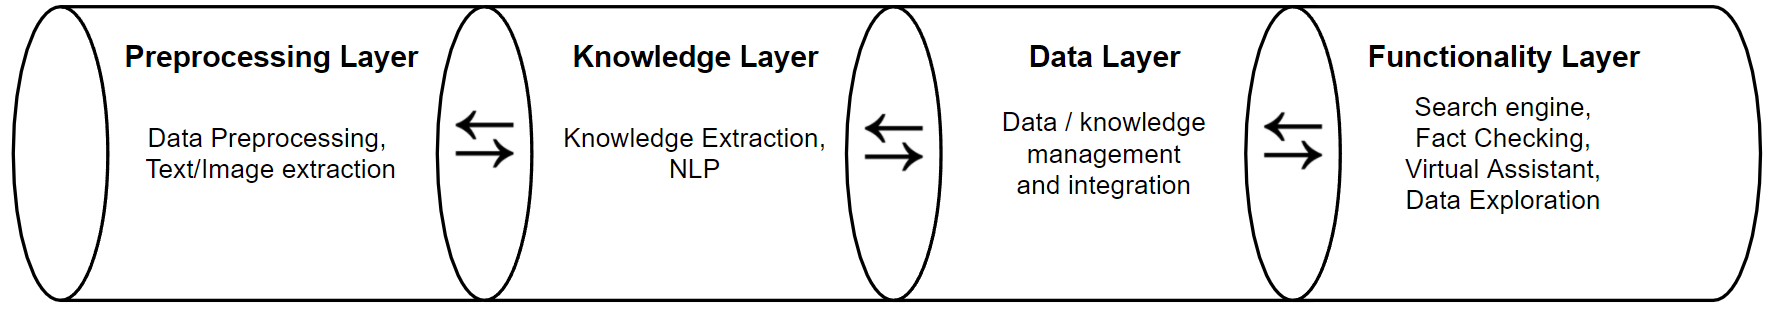
\includegraphics[width=1\textwidth]{Images/Pipeline.PNG}
    \caption{Illustration of the Knox pipeline\label{fig:pipeline}.}
\end{figure}

Last year, a User Interface (UI) layer was introduced. This year, the responsibility of creating UI elements have been split among all groups, who provide interface for their own systems.

\subsubsection{Preprocessing Layer}
The preprocessing layer is responsible for extracting data from \textit{Nordjyske Mediehus} articles and \textit{Grundfos} manuals. Many of these documents are photo scans of old articles, which means that both font, layout, and quality varies from document to document. For this reason, it is necessary to convert many of the documents to a standard format, before it is possible to extract any data. The result should allow all data from \textit{Nordjyske Mediehus} and \textit{Grundfos} to be extracted. 

\subsubsection{Knowledge layer}
The knowledge layer is used to process the data extracted by the preprocessing layer. Methods like Natural Language Processing (NLP) algorithms should be applied to extract knowledge, word count should be tallied and sent to the database, or the text should be annotated to extract entities and their relations, enabling a knowledge graph to be constructed.

\subsubsection{Data layer}\label{databaseResponsibility}
The data layer is responsible for handling the flow of data between the knowledge layer and the functionality layer in the \knox{} pipeline.
New data must be stored on the servers, and it must be accessible to the components that need it. 
This requires close cooperation with the other layers in the pipeline.


As multiple components in the \knox{} system both provide and require access to data, there needs to be a streamlined process for handling this.
In addition, both data storage and access must be handled efficiently.

\subsubsection{Functionality layer}
The purpose of the functionality layer is to use the data from the knowledge layer to apply functionality to the system.
Different kinds of functionalities can be added such as fact-checking, data exploration, search engine, and a virtual assistant.
 The goal for the functionality layer is to provide components, allowing a user to interact with the Knox system. 

\Section{Communication} 
To collaborate on the project, several communication tools were used, one being ClickUp \cite{clickup}. ClickUp was primarily used for time and task management of the different sprints for each group. In ClickUp, it is possible to create different boards and assign tasks to each board. The boards can be shared between different groups, which gives the opportunity to have a shared backlog as well as a backlog for each individual group. Hereby, the development process becomes more transparent for each group, as well as the product owner. It is also possible to mark tasks with a workload, so it is possible to see how time-consuming a task is estimated to be. ClickUp is thus an implicit communication tool, making it possible to see how far each group is. If one group has very few important, time-consuming tasks, they should be open to helping other groups, if they have an important task, which they are not able to fulfill within the sprint.
\\\\
Because of the layer structure in the project workflow, many small meetings took place during each sprint. Therefore, it was decided that a post-it note should be taped to each group room door. The note should say, which groups were located in the room, as well as which layer and project they were working on, and their typical meeting hours. 
Many of these small meetings were arranged through Slack \cite{slack}. Slack was used for all direct communication between the different groups, as well as scheduling of meetings. It was also used for knowledge sharing, such as information about which servers to use. Slack has features such as channels, threads, and direct messages, and many of these features were frequently used. Each group was given their own channel, where people of other groups could write information or questions to the members of the channel. During the sprints, several committees were formed, and each committee was also given a channel in Slack. The committees were formed as a communication path between the groups and layers. The committees were specific forums for concrete problems, concerning collaboration on the project in general. The committees will be described in more detail in \autoref{SHARED-committees}.

\section{Agile cooperation}\label{knox_collaboration}
\textit{The following section have been written in collaboration with other Knox project groups.}


\subsection{Agile approach in Knox}\label{common_agile_methods}
In the previous iteration of Knox, Scrum was used as a framework for planning in and between the project groups. It has therefore been chosen to continue to use a Scrum-inspired approach for the project. The reason why it was Scrum-inspired and not only Scrum was because many groups had not used Scrum before, and therefore some aspects were not fully realized. For example, for the first couple of sprints, there were no sprint reviews or retrospectives in the Scrum-of-Scrum meetings.  

Deviations were made from the standard Scrum to manage overhead in the Scrum-of-Scrums work environment. Multiple committees (described in \autoref{SHARED-committees}) were implemented to reduce the duration of Scrum-of-Scrums meetings and the responsibilities of Scrum masters. The goal of the committees was to assign responsibility for tasks affecting all groups.
This led to a lot of collaboration between the groups, which ensured communication and transparency. 

\subsection{Roles and Events}\label{roles_and_events}
The theory and definitions of the different Scrum terminology will not be discussed in this section. All definitions are taken from The Scrum Guide by Ken Schwaber and Jeff Sutherland
\footnote{The Scrum Guide (2020) - \url{https://Scrumguides.org/docs/Scrumguide/v2020/2020-Scrum-Guide-US}}.


The Knox project consists of eight Scrum teams, who work on different features of the pipeline. In general, a Scrum team has their own Scrum master and product owner. The “global” project owner for the whole Knox project was an older student who had worked on the previous iteration of Knox. The product owner also worked closely with the group supervisors during the project.

All groups made a backlog for the project together, however, all tasks were somewhat loosely defined, and it was up to the assigned groups to specify them. Sprint planning was done during the Scrum-of-Scrum meetings, which were held weekly throughout the project. Sprint reviews began during the third sprint and were made with a PowerPoint containing the finished and in-progress tasks of the groups. A component diagram of the Knox project was also updated each week. Sprint retrospective was held by the Scrum masters of all groups between sprints.

\subsection{Our Agile Approach}\label{our_agile_approach}
\todo{write about our own agile approach - the initial methods used and such.}

\section{Committees}\label{SHARED-committees}
\texit{The following section have been written in collaboration with other Knox project groups.}

Committees were established, as an attempt to ensure cooperation between the different groups. Several committees were founded.

\subsection{Scrum-of-Scrums}
Scrum-of-Scrums was introduced in the Knox project as a means of helping teams obtain transparency as well as the possibility to adapt to a common development process and at the same time be informed of the progress of other groups\ \cite{agile}.
The meetings were held on a weekly basis and helped ensure that the groups had a common discourse during each sprint. 
The PO was also present during meetings, in order to ensure that the decisions made would be meaningful elements in Knox. 
During the first three sprints, the main topic of the meetings was the development of an minimum viable product.
The Scrum-of-Scrums meetings helped create the above-mentioned qualities.

Scrum-of-Scrums was beneficial to the communication between teams and helped reach agreements on how to ensure that the development process was carried out in a manner that focused on cooperation between the teams.

\subsection{DevOps}
DevOps combines various practices and tools and emphasizes the importance of implementing a DevOps culture. According to a survey, 99\% of the respondents believed that using DevOps had impacted their organization in a positive way \cite{Atlassian}. Using DevOps helps improve the speed of the work process, along with communication and collaboration between teams.

The DevOps committee focused on streamlining the development process, and decisions on the use of Continuous Integration were discussed during these meetings. 
Important decisions such as “definition of done” along with requirements for code standards and the rules for server use were also discussed during these meetings.
Several of the members of the committee had zero to little experience with DevOps when starting out, hence the committee worked as a platform of information sharing and collaborating on finding the most viable solutions. This helped reach a common understanding of DevOps, as well as implementing methods such as definition of done, to ensure that the process was streamlined.

\subsection{Writing committee}
During Scrum-of-Scrums, it was agreed upon that each team would collaborate on parts of the written project. The meetings were held in order to collaborate on writing these parts, to correct the written material, and ensure that it lived up to collective standards of writing.


% Indsæt UI

%*context for the project 
%		*purpose
%		*collaborators 
%*2nd year of knox and status of project at handover
%		*Handover and PO
%		*current status
%*Goal of second year (search engine)
%		*working search engine
%		*extension of individual layers
%*tail into next section (pipeline?)
\chapter{Problem Formulation}
\section{Semester Context}
This semester is thematically based on students learning how to collaborate as teams on a complex project.

To accommodate this, students work in interdependent teams on separate parts of a complex project. 
Each team has a specific role, and should, to some degree, provide support to teams that they are collaborating with.
To this, students are taught certain software process models, and are expected to use them in their work.
This is supposed to emulate the environment of an actual software project.

We are part of the Knox multi-project. In the next section, we will describe Knox and our role in more detail.
% However, it is important to note that Knox is developed using Agile software development practices.
% This is also the process model that we will be using in this semester.
% 
% The choice to use Agile software development practices is not a technical decision, but rather a choice of a process model that is suitable for the type of work that we are doing.
% We find the benefits of an Agile approach superior to other models, considering the scope, details, and requirements for the project.
% To specify, we will be dealing with many of unknowns, which means that the flexibility of an agile approach will be beneficial.



% A case could be made for the waterfall model, in that we have a certain deadline for delivering a report, and the phases of writing the report (and the deadline) are known beforehand. 
% However, the contents of the report is what is important, and that will only become better by 1. following and learning from the designated process, and 2. doing good work, which the agile approach — in our estimation — would help us do.
% The work that we will do was, when we started the project, largely unknown.
% 
% Similarly, a case could be made for the integration and configuration model.
% We could do much of our assigned task by integrating and configuring various 3rd party components and systems. 
% However, we would like to learn as much as we can. 
% As such, the approach of using the work of others is not ideal — even if you learn a few things by implementing it.

%\section{KnoxLayer}
The knowledge engineering toolkit or Knox is a project which goal is to provide a flexible toolkit whose components can be combined to solve bigger problems. Here the long-term vision for Knox is to provide access to chatbots and personal assistants that can provide a proven answer to the users' questions through the usage of knowledge extraction, natural language processing, fact-checking, explainable ai. 
The overall goal for the 2nd iteration of Knox is to complete a search engine with the provided components from the 1st iteration. Furthermore, a shared interface for the front-end and back-end and an advancement of its components is expected. 


The Knox project itself is currently split into a 4-layered pipeline structure. The first layers of the pipeline is the Pre-processing layer which takes image files as input. Here the goal is to convert the image files into text files using optical image recognition. 


Once the first layer has completed its objective the files are then sent to the next stage of the pipeline being the Knowledge layer. The main task here is to extract as much data as possible from the files generated by the previous layer using natural language processing. Here the data is extracted in the form of RDF triples which consists of a subject, an object, and the predicate connecting them. 


Next up the 3rd layer also known as the data layer handles the data management and integration across the board. This layer is responsible for managing all the data extracted during the different stages of the pipeline and making sure it is available for the next stages when needed. 


The final stage of the pipeline is the functionality layer. This layer handles all the functionalities that are available for the end-user. These functionalities cover fact-checking and providing an explanation for the given prediction.


With an overview of the current state of the overall main objectives of the project  established a more in-depth look at the current state of the data layer is now needed to continue the development of the layer. 



\todo{Section vedr. database laget. Hvad har vi ansvar for?}
\chapter{Sprint 1}

\section{Sprint Purpose}
The initial sprint for the second iteration of \knox{} main purpose was for the teams to gather information 
about the current state of \knox{} including what was developed last semester as well as which features were 
left hanging when it came to an end last time it was run. Another goal for the sprint was to gain a 
good enough understanding of the current framework to be able to plan out the needed development steps to 
plan the implementation of a search engine during the next sprint. 
To facilitate the main purpose of the sprint, the goal for our team was to make sure that everyone had access to all the databases currently deployed on the \knox{} project. Furthermore a suitable understanding 
of the codebase and the current server structure, is needed for the next sprint.
\section{Findings}
Due to the focus of our group, the first task of the sprint was to gain access to the database to make 
sure that all the documented servers were running and had the expected data and structure. During this 
process, it was discovered that the documentation for the server structure and how to access them was
not documented properly. Therefore code and documentation from the other \knox{} groups were needed to dig out the 
required access keys to gain server access. Once the servers were accessed it was discovered that most 
of the servers were either partly empty only containing the schema for the expected data or filled up with 
mock data used last semester. From this discovery, it was concluded that the server was never fully setup 
to receive data from the previous layers in the pipeline. 


Examining the codebase handed over it was quickly deemed undocumented and untested to such a large extend 
that in context of the database setup in use a rewrite of the code seemed necessary to gain 
a better understanding and overview of the way data was handled in \knox. 


With this in mind meetings with the surrounding groups were scheduled to gain a better 
understanding of their current and future needs. A rewrite of the codebase was also deemed necessary and 
added to the backlog. This was done to facilitate one of the main requirements of this iteration, 
to improve the documentation of \knox and testing of the code in use.
\section{Retrospective}
The main goal of the research sprint was to gain access to all the currently deployed databases as well 
as gaining a suitable understanding of the deployed codebase. This goal was reach during the spring 
giving all group members database access and an overview of what was developed last time. 

This iteration discovered a lot of risk in how the documentation of the codebase and database is 
currently handled making the handover overly time-consuming as well allowing for too many 
misunderstandings due to the lack of documentation. To make sure this does not happen during the next 
handover an approach with increased focus on documentation was chosen to allow for an easier 
understanding of the database setup for the other teams using it and future handovers. 

This iteration discovered a lot of possible risk in how the documentation of the codebase and database i 
currently being handled. The approach taken last time did not involve a lot of focus on documentation 
which makes the project handover overly time-consuming as well as creating the possibilities of 
misunderstandings due to the lack of proper documentation. Due to request from the product owner to make 
sure this does not happen again an approach with increased focus on documentation was chosen. This 
approach both allows the other teams to easier understand how databases are running making it easier for 
them to usage them while also providing an easier handover next time.  



\chapter{Sprint 3\label{sec:Sprint2And3}}
%\chapter{Introduction to the search engine}
For the third sprint, the various groups of the Knox project were tasked with finishing the implementation of the Search Engine. The goal of the Search Engine is to search through files provided by \textit{Grundfos} and \textit{Nordjyske Mediehus}, using phrases or words. When the groups received the project, the Search Engine was non-functional. Issues in the different components resulted in the groups collaborating on fixing current modules or implementing new ones. Many of the problems inherited from last years' implementations were results of miscommunications between the pipeline layers. These issues mainly occurred due to inconsistency in the structure of objects sent between the different layers. Other issues included a lack of documentation and routing issues. 

The preprocessing layer experienced problems with parsing some files, as well as API communication with the knowledge layer. The knowledge layer did not have an established connection to the Data layer and could not  add the entries to the database. The data layer did not have working APIs for accessing the database and the functionality layer, therefore, accessed the wordcount database directly. At this point in time, the database only contained test data.

To settle these issues, first a product backlog, and after some time an MVP was defined for the search engine. The latter being defined as: “All non-problematic articles from \textit{Grundfos} and \textit{Nordjyske Mediehus} from 2017-2021 must be queryable from the UI in natural language, with an option for choosing which source to search in, and with a link to the original article.” 
The backlog contained tasks for each of the Knox project groups.
\section{Sprint Planning}
\subsection{Knox Goal}
The overall goal for the Knox project during this sprint was to get the search engine to work. To accomplish this goal the product owner specified a list of expectation that when completed would fufill a minimal viable product. The specified list is outlined in figure X.
\begin{itemize}
	\item It should be possible to make searches in all the available databases.
	\item It should be possible to make searches using keywords in all the available data.
	\item It should be possible to make searches in all Nordjyske articles from 2017-2021
	\item It should be possible to make searches in all the Grundfos manuals, barring those that have shown to be problematic during processing.
	\item The UI should minimally be able to display a link to the given article but preferably display the title and text.
\end{itemize}

With the overall goal for the sprint contained in figure x, a granulated sprint goal could be made that accounts for the focus of our scrum group.


\textbf{Sprint goal}
As noted in the preceding sprint, the codebase that was inherited from the previous iteration was deemed problematic and costly to maintain. Therefore our sprint goal for this iteration was based on updating the codebase to better comply with the requirements for the Knox goal.


Based on this observation as well as the aforementioned requirements, our sprint goal was as follows:


\textit{Make the minimally required amount of API endpoints available to satisfy the requirements for the search engine, and create the necessary documentation.}


\textbf{Backlog \& Increments}
The sprint goal could then be granulated into subtasks. With the tasks granulated, a session of scrum poker was held in order to evulate the time requirement of each task. Lastly the tasks were categorized by their priority and focus point and divided into three different sprint increments: Wordcount API, Write Report, Wiki Documentation. 


%%Remember to add an estimate to Write report and wiki update
\begin{table}[]
\begin{tabular}{|l|l|l|ll}
\cline{1-3}
Estimate & Increments                         & Tasks                         &  &  \\ \cline{1-3}
82       & \multicolumn{1}{c|}{Wordcount API} & CRUD operations on controller &  &  \\ \cline{1-3}
X        & Write Report                       & Document the process          &  &  \\ \cline{1-3}
X        & Wiki Update                        & Feature documentation         &  &  \\ \cline{1-3}
\end{tabular}
\end{table}





%\subsection{Sprint goal}
%The sprint goal for this group
%How does our sprint goal help with the overall sprint goal
%The purpose and priority for each increment
%Show the available backlog

\section{Increment 1.}
With the aforementioned tasks in mind, we will now move on to describing the first increment of this sprint.

We start by outlining the different database frameworks considered for the project.
Afterwards, we discuss which framework was chosen and why.


\subsection{CRUD}

As outlined in the planning for this sprint, the main focus of this sprint was to implement API end-points for the database.
As we already had a working database, the goal of this increment was to write a CRUD API in C\# such that the other layers could use to access the database via HTTP requests.
The CRUD operations we implemented are based on requests from the other layers, and what they thought they needed to retrieve from the database.
To implement this, we split the CRUD operations into three different Routes handling different aspects of the database. The routes are called: WordCount, WordRatio and Schema. Each route has its own endpoints and can access different tables in the database. The API has been split into three routes that each cover a section of the database. Wordcount is for inserting articles into the database, WordRatio is used as an absbraction over the WordRatio table in the database, and the Schema route is used to add JSON Schemas to the database.

The pipeline for the API is outlined in figure \ref{Node02Sprint3}.

\begin{figure}[h]
    \centering
    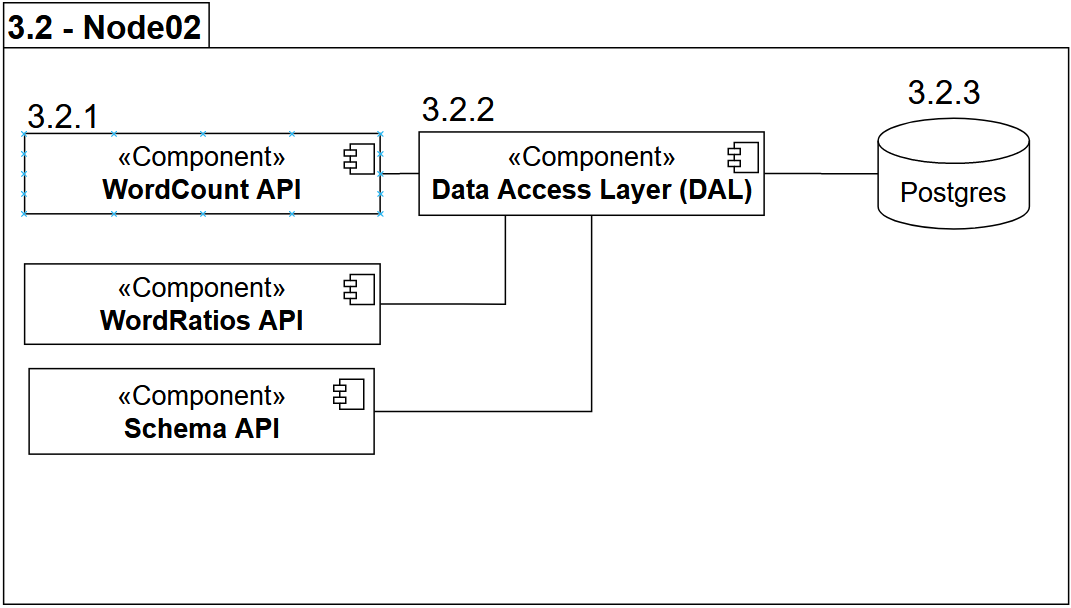
\includegraphics[width=\linewidth]{Images/Node02Sprint3.PNG}
    \caption{Node02 server pipeline in sprint 3.}
    \label{Node02Sprint3}
\end{figure}

\subsubsection{WordCount}

The first route we created was the WordCount route. It is used by the knowledge layer to insert information about an article into the database. It is also used by the functionality layer to find the filepath of an article.

In the controller we implemented 2 methods, a \texttt{GET} and a \texttt{POST} method.
\begin{table}[h]
    \begin{tabular}{|llll|}
    \hline
    \multicolumn{4}{|c|}{\textbf{WordCount}}                                                                                 \\ \hline
    \multicolumn{1}{|l|}{Name}                 & \multicolumn{1}{l|}{Method} & \multicolumn{1}{l|}{Input}       & Response on success       \\ \hline
    \multicolumn{1}{|l|}{\texttt{GetFilepath}} & \multicolumn{1}{l|}{GET}    & \multicolumn{1}{l|}{Integer}     & Article        \\ \hline
    \multicolumn{1}{|l|}{\texttt{Post}}        & \multicolumn{1}{l|}{POST}   & \multicolumn{1}{l|}{JSON Object} & Status message \\ \hline
    \end{tabular}
    \end{table}

The \texttt{GET} method called \texttt{GetFilepath}, takes a integer "id" as an argument and finds an article in the database with the given "id" and returns the articles filePath as a JsonResult if it exists, otherwise an error is sent back.


In WordCount, we also implemented a \texttt{POST} method called \texttt{Post} which takes a JSON object from the HTTP body as a parameter which should correspond to an array of articles. 
The JSON object should be valid according to a JSONschema on the database, which determines the required format of the of the JSON object and the fields needed. If the JSON object does not fit the schema, an error message is sent back. 
The articles are then checked for duplicate data on the database, if there is any it is removed and a message is added to the response that the article already exists. The remaining articles can then be inserted into the database, and a status message is returned with the potential duplicate article names. 
 
\subsubsection{WordRatio}
The WordRatio route is used by the functionality layer to fetch specific data from the database.
As the WordRatio table is a view, it cannot be used to store new data. 
The primary purpose of WordRatio is to check how many times a given word occurs in an article.
WordRatio consists of one \texttt{GET} method with an optional parameter. 
\begin{table}[h]
    \begin{tabular}{|llll|}
    \hline
    \multicolumn{4}{|c|}{\textbf{WordRatio}}                                                                                                                                           \\ \hline
        \multicolumn{1}{|l|}{Name} &
        \multicolumn{1}{l|}{Method} &
        \multicolumn{1}{l|}{Input} &
        Reponse on success \\ 
    \hline
        \multicolumn{1}{|l|}{\texttt{GetMatches}} &
        \multicolumn{1}{l|}{GET} &
        \multicolumn{1}{l|}{terms (string[]), sources (string[])} &
        WordRatio for all articles from source with term \\
    \hline
        \multicolumn{1}{|l|}{\texttt{GetMatches}} &
        \multicolumn{1}{l|}{GET} &
        \multicolumn{1}{l|}{terms (string [])} &
        WordRatio for all articles with term \\
    \hline
    \end{tabular}
\end{table}

The \texttt{GetMatches} method is used to query one or more specific words on the WordRatio table.
One may provide one or more sources in which to search for the specified words.
If no sources are provided, the database searches for the given words in all sources.
The Rows of the table matching the terms and sources.

\subsubsection{Schema}
The last route we implemented in this iteration is the Schema route which is used to post and retrieve a JSON schema from the database. These are later used to verify JSON objects as input on other endpoints. 
This schema consists of two \texttt{GET} methods and a single \texttt{POST} method.
By creating a route for fetching the validation schemas, we enable easy validation and a common understanding of the structure of input data from the knowledge layer.
\begin{table}[h]
    \begin{tabular}{|llll|}
    \hline
    \multicolumn{4}{|c|}{\textbf{Schema}}                                                                                                     \\ \hline
    \multicolumn{1}{|l|}{Name}                     & \multicolumn{1}{l|}{Method} & \multicolumn{1}{l|}{Input}               & Response on success \\ \hline
    \multicolumn{1}{|l|}{\texttt{GetSchema}}       & \multicolumn{1}{l|}{GET}    & \multicolumn{1}{l|}{SchemaName (string)} & JSON Schema         \\ \hline
    \multicolumn{1}{|l|}{\texttt{GetAllSchemas}}   & \multicolumn{1}{l|}{GET}    & \multicolumn{1}{l|}{None}                & All JSON Schemas    \\ \hline
    \multicolumn{1}{|l|}{\texttt{PostJSONSchemas}} & \multicolumn{1}{l|}{POST}   & \multicolumn{1}{l|}{JSON Schema}         & Status message      \\ \hline
    \end{tabular}
\end{table}

The first \texttt{GET} method is called GetSchema which takes a SchemaName as its input and returns a JSON Schema. 

The second \texttt{GET} method is called GetAllSchemas which takes no input and returns all stored JSON schemas. 

The last method is a \texttt{POST} method called PostJSONSchema and takes a JSON Schema as its input and inserts it into the database.
The body of the post request must consist of two fields - the schema name, which is its primary key in the database, and the schema content itself. Before the schema is inserted in the database it is checked if it is a duplicate, if that is the case an error message will be sent in response.
A schema gets stored in the database in the format known as \texttt{jsonb} or JSON binary which is a built-in type provided by \postgres{}.
This format is used to store a JSON object as binary which uses much less space than a \texttt{varchar} or regular JSON type would.
Even though \postgres{} may not be the most efficient DBMS for storing JSON data, it is sufficient for this use case, as posting and fetching Schemas will not be done often. 
\subsection{Docker}
Docker is an open source containerization platform that allows for a simplification of deliveries in distributed applications through the usage of containers.\cite{Container_Docker} 
Before giving a more detailed description of Docker, an overview of what a container is and how it is used is needed. 


Containers were originally developed to solve the issue where a program may work on one system but encounter problems when moved to a different one. 
Using containers allows developers to package their code together with its required dependencies. 
Moving around a prepackaged application with all its dependencies ensures that the software is going to run the same regardless of the infrastructure in place.\cite{Container_Docker} 


A container image is a lightweight version encapsulating everything needed to run that application. These images are then turned into containers at runtime. 
This is made possible by the build process isolation and virtualization capabilities in the Linux kernel. 
These capabilities allow for multiple application components to share the resources of single host operating system, 
in much the same way a hypervisor allows multiple virtual machines to share the same hardware resources of a single computer.\cite{Container_Docker}


Using Docker rather than a virtual machine provides the following advantages:

\begin{itemize}
    \item Lighter weight
    \item Resource efficiency
    \item Improved developer productivity
\end{itemize}

Docker itself is then used to enhance these native Linux features allowing us to automate container creation and easily move the containers between environments.\cite{Docker_IBM}
\subsection{Continuous Integration and Delivery}
In our work, we have used both Continuous Integration (CI) and Continuous Delivery (CD).
For CI, we have used GitHub with GitHub Actions. We have created a GitHub Actions workflow that
runs the tests in our project; and another one that tests the code quality. These checks run every time commits are made towards the main branch. This ensures that we keep that branch production-ready
at all times.

For CD, we have implemented an automatic deployment system that deploys the code to the production server.
We start the workflow by tagging the commit with the version number. Once we push the tag, a GitHub Actions
workflow is triggered that deploys the code to the production server.
To facilitate the deployment, we containerized our software. The Action workflow starts by building the
Docker image, which is pushed to the GitHub Package Repository. On the production server, we have a Docker 
container watching for new releases. When a new release is pushed, the container pulls the new image and
deploys it.


\section{Review}
The goal for this sprint can be seen in section \ref{ssec:sprint3Goal}. We were to implement part of the Knox Search Engine MVP, which meant that we were to facilitate data access and storage.

\subsubsection{What has been accomplished?}
This sprint, we have implemented operations for the WordCount API. This was done in close collaboration with the neighboring layers. 
Besides this, we also wrote documentation for the relevant implementation details. A full overview of what was done can be seen below.

\begin{itemize}
    \item \texttt{GET} \& \texttt{POST} API endpoints for the WordCount database.
    \item WordRatio response objects for endpoints, rather than previous layers directly querying the view.
    \item API for JSON schemas used for validating data sent to the API.
    \item API project and database containerized.
    \item Development and production environment set up and configured for rapid development \& deployment.
    \item Implemented CI/CD using Docker and GitHub Actions.
    \item Restructured database using a code-first approach.
    \item Repository-unit of work pattern has been implemented to promote encapsulation and separation of concerns.
    \item Wiki restructuring and documentation of configuration and API.
\end{itemize}

While we did manage to implement most of what was requested of us, we did not document this to the extent that our Definition of Done requires. 
We have decided to carry over these tasks to the next sprint, prioritizing them first. In the sprint retrospective, we will discuss why we did not accomplish everything we wanted to, and what we are doing about it.

Towards the end of this sprint, we demonstrated an end-to-end test to the \knox{} product owner. The pipeline seemed to work well, and we were able to get the product to work as expected. This was later confirmed by the PO. 
Six days after the end-to-end test, an API endpoint stopped working due to heavy memory load. We pushed a hotfix to fix this shortly after.

\subsubsection{What has changed in the environment?}
For this sprint, the primary focus has been to implement the Knox Search Engine. As such, all other groups have had the same focus, and therefore they have not requested anything from the database layer yet. 
We expect to see a lot of changes to the database layer in the next sprint, as some groups have mentioned that they would like to store different types of data next sprint.
A full overview of what has changed can be seen below.

\begin{itemize}
    \item The structure of the objects' sent from the below layer have changed: a 'publication' field has been introduced in the schema defining the object.
    \item We found out that the Knox Product Owner will not be creating a new backlog with tasks for us to solve, but that we should rather create meaningful tasks ourselves.
    \item We have made other groups realize that creating server-users, database schemas based on their use-cases, and similar task are their responsibility.
\end{itemize}

\subsubsection{What next?}
As mentioned before, we were asked to suggest possible next steps for our share of the Knox project. The below list encapsulates our suggestions---some of which are based upon requests from other groups.

\begin{itemize}
    \item At the Scrum of Scrum retrospect, many groups told that they want to work with knowledge graphs. Therefore, we should prepare for tasks regarding the RDF database.
    \item We should be prepared to provide assistance with the WordCount database endpoints. This included minor changes and new endpoint implementation.
    \item Potentially, we could benchmark database technologies for the Knox project, to find a good option for the Knox use-case.
\end{itemize}
\section{Retrospective}

\subsection{Reflection on the sprint}
All features planned during the sprint planning phase was implemented by the end of the sprint, but we did not document the code as well as we had initially planned. 
This clashes with our Definition Of Done, which means we did not fully reach the goal of this sprint. We have attached our Definition of Done in section \ref{sec:definitionOfDone}.

We planned out the implementation to a certain degree, but used a non-optimal format for the tasks, which led to confusion down the line. Namely, we should have described what the task encapsulated more than giving it a simple name--like 'POST'. 

We also did not use user-stories, which contributed to the confusion, as they would have otherwise provided a certain context for the tasks.

The remaining tasks were lackluster and-or nonexistent, which led to trouble doing structured writing, as we had to figure out what should be written every time we wanted to write.
    
To some extent, this was caused by conflicting information given by various sources. We also received a lot of 'urgent, but not important' tasks from other groups, which we had to react to immediately.
    
Due to the above, there were times when individual members did not exactly know what we had finished nor what other members were working on. Tasks were added almost daily, continuously changing the scope of the sprint.
As such, we did not hit our original point-estimate---it became completely irrelevant due to the rapid changes in scope.

\subsection{What we learned}\label{Whatwelearnedsprint3}
We learned that we had to be more vigilant about narrowing the scope of our tasks. 
This was especially true when working on the API's where we initially thought that we should develop full CRUD capabilities, but it turned out that only some of the capabilities were necessary. 
From this we gathered that we should use some agile method to better our understanding of the needs of different layers.

We should not change response object structure after it has been deployed---we could solve this by implementing classes that represent the response objects, instead of sending domain models. 

Intergroup communication was a big part of the sprint, as we had to work with other groups to get the right information. 
Working together while testing gave great insight into the needs of the other groups, and we were able to implement the desired features much quicker.

As the semester courses taught us more about agile methods, we found that we did a few things in a non-conventional way. Planning poker was a great way to get a sense of the scope of the sprint, but we should have used a more structured way to do it. 
Instead of the way we played in during sprint planning, we will make the following optimizations:
Each participant has a set of cards with numbers on. These numbers represent the relative sizing of a task, which is why it is common to use the Fibonacci sequence, where the numbers are well spread out.
Each round begins with the Product Owner reading a user story, which is then discussed. Then, each participant selects a card with their estimate of the task. Once every participant has selected a card, the cards are turned over. If everyone is within two cards of each other, the average of the numbers on the cards is taken as the user story estimate. If that is not the case, the outliers will discuss, and a new round commences.
This is done until there are no more user stories left\cite{sutherlandScrumArtDoing2014}.


We also learned that doing velocity analysis is a great way to know if team productivity is actually improving, which should be a result of us implementing optimizations and removing impediments.
Tasks should also not be marked as complete before they have been shipped to production, as per Scrum convention---a task is not done before it is delivered\cite{sutherlandScrumArtDoing2014}.

\subsection{How we can improve in the next sprint}

\subsubsection{Start doing}

\begin{itemize}
    \item Create user stories based on input from stakeholders
    \item Specification of the data in the database---this should be given to the other groups so fewer issues regarding CRUD operations occur
    \item Update the Kanban board frequently, so group members always are updated
    \item Change planning poker strategy:
    \subitem If everyone is within two cards of each other, just average the sum of your cards.
    \subitem If people are more than three cards apart, the high and low cards talk about why they think what they do.
    \subitem Don't estimate in hours, estimate in 'work' (relative size).
    \item Velocity analysis
    \item Component diagram versioning---we want to show the progress!
    \item Tasks are not done before they are released. We will make a lane on our Kanban board as a landing for them while they wait for deployment.
    \item Sprints changed to 2-week duration. 4 weeks is too long.
\end{itemize}

Having concluded the sprint, we will proceed to the next sprint. As mentioned earlier, we will start by documenting what we did not document during this sprint. 
Other tasks will be defined during the sprint planning process, which will be discussed in the next chapter.
\chapter{Sprint X}
%Common / Overall goal for all Knox groups

\section{Sprint Planning}
\subsection{Knox Goal}


\textbf{Sprint goal}


\textbf{Backlog \& Increments}

%The sprint goal for this group
%How does our sprint goal help with the overall sprint goal
%The purpose and priority for each increment
%Show the available backlog

\section{Increment 1.}
%Deliverable, implementation and documentation
%During tis increment we will.... description of results of the implementation and needed documentation / theory. 
%Backlog overview / fulfilment
%updated diagrams

\section{Review}
\section{Retrospective}

\chapter{Sprint 5}
%Common / Overall goal for all Knox groups

\section{Sprint Planning}\label{section:sprintPlanningSprint5}
In this sprint, we will be working on the RDF database seeing as the WordCount database is now finished.

\subsection*{User stories}\label{sec:userstories5}
The \knox{} product owner have given us two user stories, which we can use to detail the coming tasks for the sprint.
Our own product owner, along with the second and fourth layer, granulated these user stories into tasks.
This helped us understand how to accommodate the needs of the two layers and prioritize the stories.
This, in turn, helped us generate as much value to the pipeline as quickly as possible \cite{UserStories}.

\userStory{the knowledge layer}{to be able to insert Triples into a storage}{can access it later}
\userStory{the functionality layer}{to be able to query an RDF graph}{can use it in search results, fact checking and virtual assistant applications without having to worry about changes to the database}

\subsubsection*{Granulating the epics}
After talking to the functionality and knowledge layer, we found out some of the details about how they want database access to work. These requirements are specified below.



\begin{enumerate}
    \item They want it to be possible to write RDF data to the Fuseki database using the Terse RDF Triple Language (Turtle) syntax and file format \cite{TurtleFormat}.
    \item They want to be able to send SPARQL queries directly to an endpoint to fetch the data. Specifically, the route for the GET request should have a string parameter called "query" containing the SPARQL query as a string. The query will be in URL-coded format.
    \item They would prefer if the response was in XML format.
    \item They do not know the size of the data they will be querying nor have an estimation.
\end{enumerate}

At this stage we had gotten enough insight to begin work on the database, however due to the other groups not knowing exactly what they want, there was a possibility of additional tasks emerging later, which would take precedence during the sprint.


From the epics, we created a backlog. As mentioned in section \ref{Whatwelearnedsprint3}, we decided to work with a different unit of measurement for determining the size of a task.
Instead of using hours, we now estimate tasks by relative sizing - but we will keep using the Fibonacci numbers for points.

To approach the prioritization of tasks differently, we decided to apply inversion thinking \cite{InversionThinking}. This involved trying to find issues with our prioitization by imagining what would happen if we did not work on the given tasks. 

We took the items from the backlog that we defined as fulfilling our sprint goal, and tried to think about what would happen if we failed to fulfill them. 
This was done to validate the implementation tasks, as they have the most significant impact on \knox{} as a whole, making sure that they are absolutely necessary. 

\subsection*{Release planning}\label{acceptCriteriaSprint5}
The \textbf{functional requirements} include reading from and writing to the RDF database. 
The read operation should be done through an endpoint which returns the data in the XML format.
Likewise, writing should be facilitated through an endpoint which receives data in the aforementioned Turtle format.


The \textbf{non-functional requirement} for this sprint is simply that the reading and writing operations should be reasonably fast such that an acceptable amount of tuples can be queried within a feasible amount of time.


The \textbf{acceptance criteria} is that the aforementioned functional and non-functional requirements must be met before this feature is deemed acceptable. 


With the planning phase completed, we now have a backlog and a MVP to which we will now begin implementing.
\section{Review}
The goal for this sprint was to implement functionality to support the user stories defined in section \ref{userstories}. 

\subsubsection*{What has been accomplished?}
Two of the three user stories have been implemented, but none of them have yet to be deployed to the \knox pipeline.
We have implemented functionality to fetch from Virtuoso through an API endpoint. The endpoint is written in C\#, and takes a query in SPARQL format. 

\subsubsection{What has changed in the environment?}
During the sprint, we discovered that many better solutions for RDF data storage exists. Therefore, the group chose to not implement an endpoint to the Fuseki service, but implement Virtuoso instead. 

\subsubsection*{What next?}
The PO has informed us that he will not give any of the \knox groups more assignments regarding the pipeline. 
For the next sprint, we will continue on the remaining user story, and deploy the endpoint for the database, as to complete the user stories. 
However, each of the knox groups must implement a UI element, and we would like to restructure the database design in the WordCount database, as discussed in section \ref{DatabaseRedesign}.

\begin{itemize}
    \item Create a simple UI element for the \knox website.
    \item Finish implementation of the last user story.
    \item Deploy the API endpoint for the RDF database.
\end{itemize}
\section{Retrospective}
We have received three user stories from the PO, but have not deployed functionality that satisfies any of them to the \knox{} pipeline. Thus, we have not completed the sprint goal.

\subsection{Sprint goal}
The goal of this sprint was to provide endpoints for an RDF database such that the \knox{} pipeline could fetch data using a SPARQL query, and input data in turtle format. We, however, did not have time to deploy the APIs despite having finished the implementation. Fortunately, the functionality layer was not ready to fetch data at this stage, which meant that the only consequence was that we did not meet our own acceptance criteria (see section \ref{acceptCriteriaSprint5}).

\subsection{Reflection on the sprint}
The report writing during this sprint took longer than initially intended and its high priority meant that we did not have as much time for other work.
The decision to switch from Fuseki to Virtuoso happened early enough in the sprint that the time waste was minimal. The time spent researching how to use Fuseki, however, was wasted due to it no longer being needed.

During the first sprints of the project, our PO did not give us any user stories. Having user stories for this sprint greatly improved our focus when grooming the backlog, and also help give us a concrete idea of when a task was done. 
The user stories for the sprint planning allowed us to granulate them with the other layers, which in turn allowed us to remove an unnecessary task. Originally, the PO did not want the endpoints to take SPARQL requests as their input.
The knowledge layer, who needed the endpoints, disagreed, and after a conversation with the PO, it was established that endpoints receiving SPARQL queries as a string would be sufficient.

\subsection{What we learned}
We have learned that report writing in pairs improves the quality of the report written. This also has the added advantage of minimizing the time spent on reviews due to the initial versions being of a higher quality.
It was also realized that using the GitHub feature that allows us to request specific people to do a review would greatly optimize our time usage. 
This is because it minimizes the amount of people reviewing the same request in case changes are needed, while also allowing us to request reviews from team members with expertize in the subject area.
Ultimately, the result is better time usage and a higher product quality. 

\subsection{How can we improve in the next sprint}
\subsubsection{Start doing}
\begin{itemize}
    \item Request reviews from specific people on GitHub.
    \item Start referencing the data written database theory
\end{itemize}
\subsubsection{Continue doing}
\begin{itemize}
    \item Pair writing
\end{itemize}

With the retrospective for sprint 5 completed the sprint planning for the next sprint can now begin. 





% \chapter{Introduction}\label{ch:introduction}
Here is the introduction. The next chapter is chapter~\ref{ch:ch2label}.


a new paragraph


\section{Examples}
You can also have examples in your document such as in example~\ref{ex:simple_example}.
\begin{example}{An Example of an Example}
  \label{ex:simple_example}
  Here is an example with some math
  \begin{equation}
    0 = \exp(i\pi)+1\ .
  \end{equation}
  You can adjust the colour and the line width in the {\tt macros.tex} file.
\end{example}

\section{How Does Sections, Subsections, and Subsections Look?}
Well, like this
\subsection{This is a Subsection}
and this
\subsubsection{This is a Subsubsection}
and this.

\paragraph{A Paragraph}
You can also use paragraph titles which look like this.

\subparagraph{A Subparagraph} Moreover, you can also use subparagraph titles which look like this\todo{Is it possible to add a subsubparagraph?}. They have a small indentation as opposed to the paragraph titles.

\todo[inline,color=green]{I think that a summary of this exciting chapter should be added.}

% \chapter{Chapter 2 name}\label{ch:ch2label}
Here is chapter 2. If you want to leearn \todo{I think this word is mispelled} more about \LaTeXe{}, have a look at\cite{Madsen2010}, \cite{Oetiker2010} and\cite{Mittelbach2005}.
\missingfigure{We need a figure right here!}


% \chapter{Conclusion}\label{ch:conclusion}
The code that we overtook from last year for the search engine was incomplete and did not work.
We therefore implemented the database from scratch using C\# and the Entity Framework Core.
Our first attempt at this went well as is fulfilled the requirements provided by the Product Owner. 
This was verified through an end to end test where all layers participated.
However, despite this, the design had a major flaw in terms of excessive memory consumption. 
Fortunately, near the end of the project, we were able to allocate time to a redesign which addressed this problem.
We were unable to create a BCNF design on time though, and we therefore believe that the database group next year should prioritize this.

The solution from last year used to store RDF data was deemed problematic.
It required periodic restarts in order to move the data from in memory into persistent disk storage.
Therefore, a large effort was made into building a new system for handling the \knox{} RDF data storage needs. 
Here, Virtuoso was deemed as an appropriate framework since it lived up to the requirements provided from the other layers. 

Both databases were tested using Postman to ensure that the endpoints work as intended.
A few unit tests were also written for JSON validator, however the database functionality itself remains largely untested as we cannot, and should not, test a framework.

The main purpose of this semester project was to obtain knowledge and experience in analysis, design, implementation and evaluation of complex software systems in a large development environment \cite{AAULearningGoals5thSemester}.
Due to different understandings of agile and scrum, however, conflicts and problems arose intermittently.
Several committees were created whose purpose was to dictate specific guidelines or be responsible for certain aspects.
Some groups disagreed with the decisions made by those committees, and as there was no concrete project lead, nothing could truly be enforced. 
The lack of a project lead also meant that suggestions and complaints from groups resulted in little to no changes.


Another goal of this semester was to learn proper version control and module encapsulation, however this idea fell short due to the complete lack of security for the \knox{} repositories. 
Any group could simply force code into other groups' repositories, which caused time-consuming conflicts to occur.
In addition, other groups would suddenly request new features that needed to be implemented urgently.


Consequently, due to the aforementioned structural and management issues, it was difficult to follow a concrete sprint planning structure.


Ultimately, we feel as though the concept of \knox{} is good, however the execution was unfortunate. 
While we did learn a lot, the rough nature of the project and its conflicts have resulted in division among students. 
Internally, the structure of \knox{} resulted in a productive workflow for the group as a whole. 
We believe that the positive workflow we experienced internally may also flourish across group collaboration in future projects when these issues have been addressed.
% If you do not write the report in English, translating the bibliography title to, e.g., Danish, should not be done here. Instead, you should change the main language in the preamble (look for the line \usepackage[danish,english]{babel} and change the order/delete the 'english' option). See more in the babel package documentation.
\printbibliography[heading=bibintoc, title=Bibliography]
\label{bib:mybiblio}
\appendix
\chapter{Appendix A name}\label{ch:appAlabel}
Here is the first appendix

\chapter{Data access models}\label{AppDataAccess}
% % JsonSchemaModel
\begin{figure}[H]
    \centering
    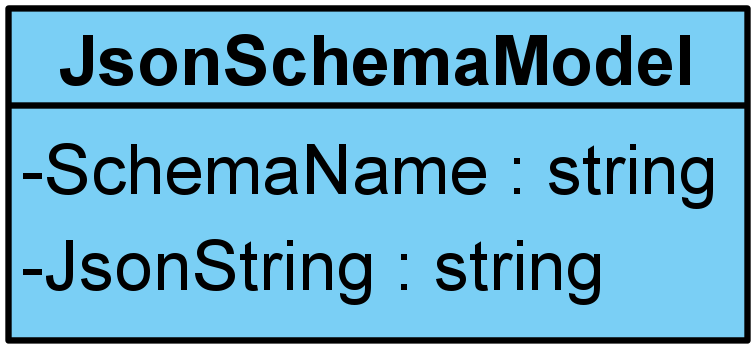
\includegraphics[scale=0.25]{Images/JsonSchemaModel.png}
    \caption{The model of the \texttt{JsonSchema} table.}
    \label{JsonSchemaModel}
\end{figure}
% WordRatio
\begin{figure}[H]
    \centering
    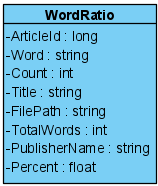
\includegraphics[scale=0.25]{Images/WordRatioModel.png}
    \caption{Diagram of WordRatioModel.}
    \label{WordRatioModel}
\end{figure}
\end{document}
